%\documentclass[]{dinel-upm}
\documentclass[a4paper,twoside,12pt]{book}
%\setlength{\columnsep}{0.7cm} % space between columns
\usepackage{filecontents}
\usepackage{gensymb}

\usepackage{lipsum}
\usepackage{fancyhdr}
\usepackage{titlesec}
\usepackage[spanish,es-tabla]{babel}
\usepackage[utf8]{inputenc}
\usepackage{amsmath,amssymb,amsthm}

\usepackage{afterpage}
\usepackage[left=2.5cm,right=2.5cm,top=3cm,bottom=2.5cm]{geometry}
\usepackage{tocloft}
\usepackage{enumerate} 
\usepackage{tikz}
\usetikzlibrary{shapes,arrows}

\usepackage{wrapfig}
\usepackage{graphicx,tabularx}
\usepackage{eurosym}
\usepackage{multicol}
\usepackage{multirow}
\usepackage{rotating}
\usepackage{pdfpages}
\usepackage{pdflscape}
\usepackage{booktabs}
\usepackage[hyphens]{url}
\usepackage{ragged2e}
\usepackage{caption}
\DeclareCaptionListFormat{myfmt}{#1.#2}
\usepackage[list=true,listformat=myfmt]{subcaption}

%\usepackage{tikz}
\usepackage[cuteinductors,americanvoltages,americancurrents,american]{circuitikz}

\newcommand{\newItemUrl}[1]{\href{#1}{#1}}
\newcommand{\tabitem}{~~\llap{--}~~}
\newcommand{\newItem}[1]{\multicolumn{3}{|p{11cm}|}{\tabitem #1}\\}

\newcommand\Tstrut{\rule{0pt}{2.6ex}} 
\newcommand\Zstrut{\rule{0pt}{3.2ex}} 
\newcommand\Bstrut{\rule[-0.9ex]{0pt}{0pt}}
\newcommand{\HRule}{\rule{\textwidth}{0.1mm}} 		
\usepackage{hyperref}
					% horizontal line and its thickness

\titleformat
{\chapter} % command
[hang] % shape
{  \normalfont\bfseries\Huge} % format
{} % label
{0.5ex} % sep
{
%	\centering 
} % before-code
[] % after-code

%nuevo comando

\newcommand{\tb}[1]{\textcolor{blue}{#1}}
\usepackage[english]{cleveref} %con este paquete si usas \cref{label} te pone automáticamente figura,ecuacion..

\Crefname{figure}{Fig.}{Figs.}% {<type>}{<singular>}{<plural>}

\newcommand{\refAnexo}[1]{(Anexo \ref{#1})}
\newcommand{\refFigura}[1]{(Figura \ref{#1})}
\newcommand{\refApartado}[1]{(Apartado \ref{#1})}
\title{\textbf{Kit de desarrollo y validación de algoritmos de control de actitud para cuadricópteros}}

\author{Miguel Fernández Cortizas}
\date{}

\newcommand{\grad}{$^{\circ}$}
\usetikzlibrary{babel}
\usepackage{tikz}
\usetikzlibrary{matrix,chains,positioning,decorations.pathreplacing,arrows}

\usepackage{pgfplots}
\usepackage{ifthen}

\usepackage{amsmath}
\DeclareMathOperator{\sigm}{sigm}
\newcommand{\diff}{\mathop{}\!\mathrm{d}}

\usepackage{fancyhdr}

\fancyhf{}
\fancyhead[LE,RO]{\nouppercase{\rightmark}}
\fancyfoot[LE,RO]{\thepage}
%\fancyhead[LO,RE]{\nouppercase{\leftmark}}

\fancypagestyle{plain}{%
	\fancyhf{}% clears all header and footer fields
	\fancyfoot[LE,RO]{\thepage}%
	\renewcommand{\headrulewidth}{0pt}%
	\renewcommand{\footrulewidth}{0.0pt}
}

     

\newenvironment{dedication}
{%\clearpage           % we want a new page          %% I commented this
	\thispagestyle{empty}% no header and footer
	\vspace*{\stretch{1}}% some space at the top
	\itshape             % the text is in italics
	\raggedleft          % flush to the right margin
}
{\par % end the paragraph
	\vspace{\stretch{3}} % space at bottom is three times that at the top
	\clearpage           % finish off the page
}

\begin{document}
	
	\pagestyle{empty}
	\pagenumbering{gobble}
	
	\begin{landscape}
	
\includepdf[page=-,angle=90]{portada/PORTADA_Trabajo_Fin_de_Master.pdf}
	\end{landscape}
	\clearpage\null\newpage

	
\begin{center}
	\textbf{ UNIVERSIDAD POLITÉCNICA DE MADRID }\\
	ESCUELA TÉCNICA SUPERIOR DE INGENIEROS INDUSTRIALES\\
	\tb{GRADO EN INGENIERÍA EN TECNOLOGÍAS INDUSTRIALES}
	
	
	\vspace{1cm}
	
	
\includegraphics[height = 10cm]{portada/logoupm}
	
	\vspace{1cm}
	
	{\LARGE \tb{KIT DE DESARROLLO Y VALIDACIÓN DE}}
	\\
	
	\vspace{0.2cm}
	{\LARGE	\tb{ALGORITMOS DE\ CONTROL DE ACTITUD}}
		 \vspace{0.2cm}
		 \tb{{\LARGE PARA CUADRICÓPTEROS.}}
	
	\vspace{2cm}
	
	{\Large Miguel Fernández Cortizas}\\
	
	
	
	
	\vspace{2cm}
	
	{\large  Tutor académico:}\\
	\vspace{0.2cm}
	{\Large D. Pascual Campoy Cervera }
	
	\vspace{0.5cm}
	
	
	\vfill{\Large Madrid - Espa\~{n}a\\
		2020}

\end{center}
\newpage


	\clearpage\null\newpage

\begin{dedication}
	En memoria de mi padrino Juan, \\
	seguiré trabajando hasta alcanzar las metas\\
	que me hubiese gustado celebrar contigo. 
\end{dedication}

	\justify
	\pagestyle{empty}
	
\chapter*{Agradecimientos}

En primer lugar, quiero darle las gracias a Carmen, por impulsarme a ser mejor persona día tras día con su cariño y su apoyo.

Asimismo, quiero darle las gracias Pascual Campoy por ofrecerme la oportunidad de trabajar y aprender dentro del CVAR y por brindarme la oportunidad de conocer a muy buenos compañeros, los cuales me han motivado, con su pasión y esfuerzo, a continuar trabajando en mundo de la investigación.

Finalmente me gustaría dar las gracias a Carlos Redondo, compañero y amigo con el que he compartido grandes momentos estos años de universidad y con el que he trabajado mano a mano en incontables ocasiones, apoyándonos y motivándonos mutuamente. 





	\pagestyle{empty}			
	\chapter*{Resumen ejecutivo}
\section*{Introducción}

Los pequeños multirrotores no tripulados (comúnmente llamados drones) son vehículos cuya popularidad en el mundo de la industria es cada vez mayor, siendo utilizados para realizar tareas en campos muy diversos, como la inspección industrial, la industria cinematográfica o para su uso en operaciones de búsqueda y rescate. Aunque la inmensa mayoría del uso de estas aeronaves es mediante teleoperación, el auge de estas aeronaves han llevado a la comunidad robótica hacia el desarrollo de sistemas capaces de realizar tareas de forma autónoma.

Con el ánimo de impulsar el desarrollo de las tecnologías necesarias para conseguir mejorar la autonomía de estos drones, existen diversas competiciones internacionales como el IARC (International Aerial Robotics Competition), IMAV (International Micro Air Vehicle Competition) o MBZIRC (Mohamed Bin Zayed International Robotics Challenge), en las que el objetivo es conseguir que las aeronaves sean capaces de realizar pruebas complejas de forma autónoma. 

Dentro de estás competiciones internacionales, existen las carreras de drones autónomos, como ADR o AlphaPilot, en las que el objetivo es que un dron sea capaz de recorrer un circuito de forma autónoma en el menor tiempo posible.

\section*{Alcance}
Los objetivos de este trabajo consisten en diseñar un sistema autonómo, para que un cuadricóptero sea capaz de recorrer un circuito de carreras de forma satisfactoria y en diseñar un controlador capaz de conseguir que un cuadricóptero vuele a altas velocidades a través de un circuito, así como generar las trayectorias que el aeronave debe seguir para recorrer el circuito de forma óptima. Adicionalmente, los algoritmos están diseñados para ser ejecutados en un ordenador a bordo, por lo que se deben optimizar para obtener el mayor rendimiento.
El desarrollo y validación del trabajo se realizará el simulador y las reglas empleadas en la prueba virtual clasificatoria del AlphaPilot2019.
\section*{Solución realizada}
\begin{itemize}
\item \textbf{Controlador:}
Para conseguir que el cuadricóptero recorra el circuito a altas velocidades se han implementado dos controladores, uno linealizado en torno al punto de equilibrio, en los que la orientación del cuadricóptero varía un pequeño ángulo respecto al estado de hover y otro para cuando esta variación es de un gran ángulo.

\item \textbf{Generación de trayectorias:} Se ha dividido la generación de trayectorias en dos partes:
Una trayectoria que abarca todo el recorrido del circuito y otra más corta dentro de un horizonte temporal próximo a la posición del cuadricóptero. Ambas son trayectorias óptimas, generadas por \textit{splines}.

\item \textbf{Arquitectura del sistema:} Los algoritmos de control y generación de trayectorias se han integrado dentro de una arquitectura modular empleando el \textit{framework} de robótica ROS. Adicionalmente se han desarrollado módulos de percepción y estimación de estado empleando datos provistos por el simulador.

\end{itemize}
	

\section*{Experimentación y resultados.}

Para realizar los experimentos se ha empleado el entorno de simulación Flightgoogles \cite{guerra2019flightgoggles}  el cual fue el empleado para las pruebas clasificatorias virtuales del Alphapilot 2019. Durante el transcurso del trabajo se han realizado experimentos para la evaluación de los controladores implementados, en los que se prueba el rendimiento de los mismos recorriendo trayectorias sencillas a distintas velocidades. Asimismo, se han realizado experimentos recorriendo el circuito de carreras entero, en los que se prueba el rendimiento del generador de trayectorias y de la arquitectura diseñada.

En estos experimentos se puede observar como el controlador para grandes ángulos es capaz de alcanzar velocidades más altas (hasta 11 m/s) con un menor error de seguimiento que el controlador linealizado. La arquitectura presentada es capaz de recorrer el circuito entero de forma satisfactoria en 24 segundos, tiempo que se encuentra dentro de los 3 mejores tiempos obtenidos por los equipos participantes en las clasificatorias del AlphaPilot2019 \cite{guerra2019flightgoggles} \footnote{Estos resultados fueron presentados en el Workshop  \textit{Perception and Control for Fast and Agile Super-Vehicles} de la conferencia RSS20, integrando los módulos de percepción y estimación de estados desarrollados por Carlos Redondo Plaza}. Un vídeo mostrando el funcionamiento del sistema en simulación se puede encontrar en \url{https://vimeo.com/428975020/80051cd0d8}.


\section*{Conclusiones y trabajo futuro}

Se ha conseguido desarrollar sistema modular capaz de recorrer un circuito de carreras de forma autónoma de forma satisfactoria. El controlador implementado permite realizar trayectorias a velocidades muy elevadas, aunque para conseguir disminuir el error de seguimiento sería posible emplear un controlador MPC que sea capaz de mitigar los cambios bruscos en las referencias. Finalmente, la decisión de dividir la generación de trayectorias en dos partes ha permitido computar ambas trayectorias a una alta frecuencia siendo capaces de adecuarse correctamente a los cambios en las estimaciones de las posiciones de las puertas en el circuito. En versiones futuras, sería conveniente tener en cuenta restricciones espaciales en la generación de las mismas.

La arquitectura propuesta permite su extensión con nuevos módulos de forma sencilla, por lo que se podría emplear para realizar otras tareas mediante la integración de los módulos necesarios.

\newpage
\section*{Palabras clave}
UAV, cuadricóptero, modelado dinámico, teoría de control, generación de trayectorias, sistemas autónomos.

\section*{Códigos UNESCO}
\begin{itemize}
	\item[] $120326$ \quad SIMULACIÓN
	\item[] $330104$ \quad AERONAVES
	\item[] $330412$ \quad DISPOSITIVOS DE CONTROL
	\item[]	$330118$ \quad ESTABILIDAD Y CONTROL
	\item[] $330417$ \quad SISTEMAS EN TIEMPO REAL 
		

\end{itemize}
\newpage
\cleardoublepage
	
	\tableofcontents
%	\cleardoublepage\null\newpage
	
	\pagestyle{fancy}
	\justify
	\pagenumbering{arabic}
	\setcounter{page}{0}
	\thispagestyle{empty}
	
	\chapter{Introducción}


El auge de los pequeños multirrotores no tripulados (comúnmente llamados drones) en diversos ámbitos ha crecido de forma exponencial durante estos últimos años. Se puede observar la presencia de estos drones en diversos ámbitos como: el industrial, para realizar inspecciones en lugares de difícil acceso o en lugares peligrosos, el cinematográfico, para grabar escenas aéreas, o para dispositivos de búsqueda y rescate, en los que se emplean para poder barrer grandes áreas en búsqueda de personas desaparecidas, entre otros. Además, dentro del mundo del entretenimiento, las carreras de drones comienzan a hacerse un hueco en países como los Estados Unidos, donde las carreras de drones son un deporte que se retransmite en algunos canales de televisión. 

Actualmente, en la mayoría de estas competiciones, los drones están pilotados por un humano, aunque recientemente, empiezan a aparecer carreras de drones autónomos, en los que las aeronaves tienen que recorrer el circuito entero de forma autónoma sin la intervención de un humano. Algunos ejemplos de estas competiciones serían: la \textit{Autonomous Drone Race} (ADR), que se celebra anualmente dentro de la conferencia de robótica internacional  IROS, o más recientemente AlphaPilot, una carrera de drones autónomos organizada por la \textit{Drone Racing League} y la empresa \textit{Lockheed Martin} con un gran premio de 1 millón de dólares para el ganador.

\begin{figure}[htb!]
	\centering
	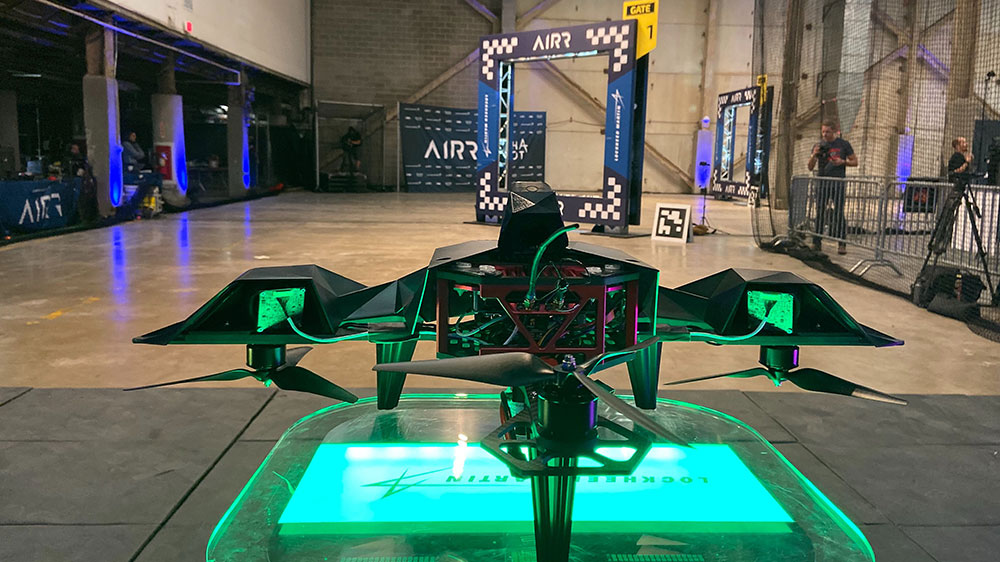
\includegraphics[width=0.80\textwidth]{imagenes/foehnAlphaPilot}
	\caption{Cuadricóptero empleado en el AlphaPilot 2019, mirando hacia la primera puerta del circuito \cite{foehn2020alphapilot}}
	\label{}
\end{figure}


Actualmente, el rendimiento obtenido por los drones de carreras autónomos aún está lejos de alcanzar el de los pilotos humanos. Es por esto que el afán por superar el nivel de los pilotos humanos es una motivación para los grupos de investigación por todo el mundo. El desarrollo de drones autónomos es un campo de estudio exigente que involucra el desarrollo de la tecnología existente en diversos campos de la robótica como: la estimación, el control, la generación de trayectorias o la percepción, entre otros. 

\section{Motivación}

El desarrollo de un sistema capaz de recorrer un circuito de forma autónoma sin interacción externa con cierta incertidumbre sobre el entorno, es un problema apasionante debido a las elevadas velocidades de vuelo y la limitada capacidad computacional, que exigen tener algoritmos de percepción y de estimación de estado más precisos y rápidos, así como algoritmos de planificación y de control más rápidos y ligeros, que permitan realizar cálculos a tiempo real.

Los avances obtenidos en diversos campos de la robótica durante el desarrollo de estos drones autónomos de carreras se pueden extrapolar para mejorar el rendimiento de los drones autónomos empleados para realizar distintas tareas con una mayor relevancia como pueden ser la aplicaciones industriales o como aquellas relacionadas con la búsqueda y rescate.

Los últimos avances en las plataformas de simulación enfocadas al desarrollo de sistemas de control de drones autónomos, como el simulador fotorrealista FlightGoggles desarrollado por Guerra et al \cite{guerra2019flightgoggles} empleado durante las pruebas clasificatorias del AlhpaPilot 2019, permiten probar el rendimiento de un sistema autónomo de forma realista y segura.



\section{Objetivos}
El objetivo propuesto consiste en diseñar la arquitectura de un sistema modular capaz de controlar un cuadrirrotor a través de un circuito de carreras de forma autónoma.

Debido a la gran complejidad que presenta el desarrollo completo de todos los módulos que intervienen en un dron de carreras autónomo, se han simplificado el desarrollo de los módulos de estimación de estado y de percepción del circuito, empleando datos provistos por el simulador. Es por esto que el trabajo se ha centrado en el desarrollo de la arquitectura del sistema y en el desarrollo de los módulos de control y generación de trayectorias, los cuales deben ser capaces de generar y seguir trayectorias agresivas a lo largo de todo el circuito a altas velocidades y con incertidumbre sobre el recorrido en sí.

Para el algoritmo de control se han implementado dos controladores del estado del arte, un controlador para orientaciones del aeronave con ángulos pequeños y otro para grandes ángulos y se ha comparado el rendimiento de ambos en el seguimiento de diversas trayectorias.

En cuanto a la generación de trayectorias, se ha optado por generar trayectorias polinómicas óptimas de tipo \textit{spline}. Para poder mejorar la capacidad de reacción del aeronave ante cambios en el circuito se ha dividido la generación de trayectorias en dos partes: la generación de una trayectoria completa a través de todo el circuito (largo plazo) y la generación de una trayectoria corta entorno a un horizonte temporal próximo a la posición del aeronave (corto plazo).

Para desarrollar los algoritmos y comparar el rendimiento del sistema realizado, se ha utilizado el simulador FlightGoogles, el cual fue empleado para las pruebas clasificatorias del AlphaPilot 2019 como entorno de pruebas.


%Este sistema estará formado por 3 partes principales:
%\begin{itemize}
%	\item \textbf{Estimación de estado:} Para poder recorrer el circuito es necesario tener una estimación precisa del estado de la aeronave a lo largo del tiempo. Para poder localizar el desarrollo de los 2 bloques posteriores se empleará la estimación provista por el simulador.
%	\item \textbf{}
%	\item \textbf{Generación de trayectorias:}
%\end{itemize}

Para poder llevar a cabo el desarrollo del trabajo de forma adecuada es conveniente desgranar los objetivos principales en tareas de alcance más reducido:

\begin{itemize}
	\item \textbf{Modulo de control}	
	\begin{itemize}
		\item Modelado dinámico del comportamiento de un cuadricóptero.
		\item Estudio del estado del arte acerca de los algoritmos de control más relevantes en las carreras de drones.
		\item Desarrollo teórico de los algoritmos de control para ángulos pequeños ($\phi,\theta  < \pi/6$) y para ángulos grandes ($\phi,\theta  \ge \pi/6 $) .
		\item Implementación de ambos algoritmos dentro del módulo de control.
		\item Ajuste de los parámetros de los controladores.
		\item Evaluación del rendimiento de ambos controladores en un entorno simulado.
				
	\end{itemize}

	\item \textbf{Generación de trayectorias}	
	\begin{itemize}
		\item Estudio del estado del arte acerca de los métodos de generación de trayectorias más empleados.
		\item Desarrollo teórico de los algoritmos de generación de trayectorias que se van a emplear.
		\item División del módulo generador de trayectorias en corto y largo plazo.
		\item Implementación de los algoritmos de generación de trayectorias empleados.
		\item Evaluación del rendimiento de los generadores de trayectorias mediante el recorrido del circuito de carreras en simulación.
	\end{itemize}

	\item \textbf{Arquitectura del sistema}	
	\begin{itemize}
		\item Estudio de las arquitecturas empleadas por los ganadores de las diversas competiciones de drones autónomos.
		\item Descomposición del sistema en los distintos módulos separados que compondrán la arquitectura final.
		\item Implementación de los módulos de estimación y percepción partiendo de las mediciones provistas por el simulador.
		\item Evaluación del funcionamiento completo de la arquitectura mediante el recorrido del circuito simulado. 
		
	\end{itemize}
	
	
\end{itemize}
	\chapter{Estado del arte}

Para contextualizar el trabajo desarrollado dentro del campo de las carreras de drones autónomos es necesario conocer los avances obtenidos por la comunidad robótica. Debido a que los contenidos del trabajo se han enfocado, principalmente, en torno al controlador y a la generación de trayectorias se ha profundizado en el estado del arte de estos campos enfocados a los drones de carreras. Adicionalmente, debido al objetivo del trabajo de generar un sistema coordinado, también se ha revisado el trabajo realizado por los finalistas de las carreras de drones autónomos más importantes.

\section{Control y generación de trayectorias}

En la primera década de los 2000, la mayoría del trabajo realizado con multirrotores empleaba controladores linealizados en torno al punto de equilibrio (\textit{hover}), los cuales, unicamente garantizan la estabilidad de la aeronave para pequeños ángulos de \textit{pitch} y \textit{roll} \cite{hoffmann2008quadrotor}. En cuanto a las trayectorias generadas, la mayoría de ellas son trayectorias polinómicas del tipo \textit{spline}, generadas interpolando una función entorno a los puntos de paso deseados \cite{vanek2005}\cite{barrientos2009}.

En 2008 V. Raffo et al. \cite{MPCRaffo2008} emplearon una estructura de control basada en un controlador predictivo basado en el modelo (MPC) que se encargaba de seguir la trayectoria y un controlador $\mathcal{H}_\infty$ que controlaba la rotación de la aeronave. Con esta estructura son capaces de seguir trayectorias sencillas de forma robusta ante perturbaciones.

En 2010, Guillula et al. \cite{gillula2010design} diseñaron un controlador capaz de realizar maniobras acrobáticas, como una voltereta hacia atrás, con un cuadricóptero de forma segura. Para ello emplearon un \textit{framework} para el diseño de regiones de cambio seguras, en las que cada región presenta un modelo dinámico distinto. Sin embargo, estas maniobras se generan de forma discontinua, necesitando analizar cada parte de la trayectoria de forma independiente y generar situaciones de cambio entre estos modos de forma segura. 

En 2011, Mellinger et al. \cite{MinimunSnap2011} presentan un controlador para cuadricópteros que permite realizar maniobras agresivas en un espacio tridimensional de forma continua. Este controlador no está linealizado en torno a ningún punto de funcionamiento, por lo que permite seguir trayectorias agresivas con un bajo error de seguimiento aunque el aeronave tenga ángulos grandes de \textit{roll} y \textit{pitch}. Este es uno de los controladores más usados actualmente debido al rendimiento que consigue con un algoritmo sencillo y con un bajo coste computacional.

En 2012, Mallikarjunan et al. \cite{mallikarjunan2012l1} diseñaron un controlador de actitud adaptativo, aplicando control $\mathcal{L}_1$, capaz de seguir trayectorias de forma precisa y robusta, con presencia de incertidumbres en el modelo de la aeronave y de las perturbaciones del entorno.

En 2016, Kamel et al. \cite{KamelMPC2016} comparan el rendimiento de dos MPCs, uno lineal y uno no lineal, en el seguimiento de trayectorias agresivas con un cuadricóptero. En estos experimentos observaron que, aunque ambos controladores eran capaces de seguir las trayectorias de forma satisfactoria, el controlador no lineal, conseguía un rendimiento ligeramente superior.

En 2017, Faessler et al. \cite{Faessler17ral} emplearon control LQR considerando tanto la dinámica del cuadricóptero, como la dinámica aislada de cada rotor. Además, consideran los limites de los rotores para priorizar la saturación de aquellas entradas que son relevantes para la estabilización del cuadricóptero. Asimismo, en 2018 \cite{Faessler18ral}, refinaron el controllador de Mellinger et al. considerando el arrastre (\textit{drag}) de los rotores dentro del modelo dinámico del cuadricóptero, en lugar de considerarlo como una perturbación externa desconocida, consiguiendo una ligera mejora en el seguimiento de trayectorias a alta velocidad.
 
En 2018, Falanga et al. \cite{falanga2018pampc} presentan un controlador MPC consciente de la percepción, el cual unifica el control y la planificación para satisfacer objetivos de acción y percepción de forma simultánea. Las trayectorias generadas por el MPC deben tener en cuenta ambos objetivos, para conseguir realizar maniobras complicadas mientras maximizan la visibilidad de puntos de interés por la aeronave.


\section{Carreras de drones autónomos}
Ganaron la competición IROS 2018 Autonomous Drone Race \cite{BeautyAndTheBeast}.

Recientemente \cite{foehn2020alphapilot}





	\chapter{Modelado de un cuadricóptero}

Un cuadricóptero es un robot aéreo con 6 grados de libertad (3 rotacionales y 3 traslacionales) y 4 motores, al tener menos motores que el número de grados de libertad, se dice que es un sistema subactuado.

\begin{figure}[htb!]
	\centering
	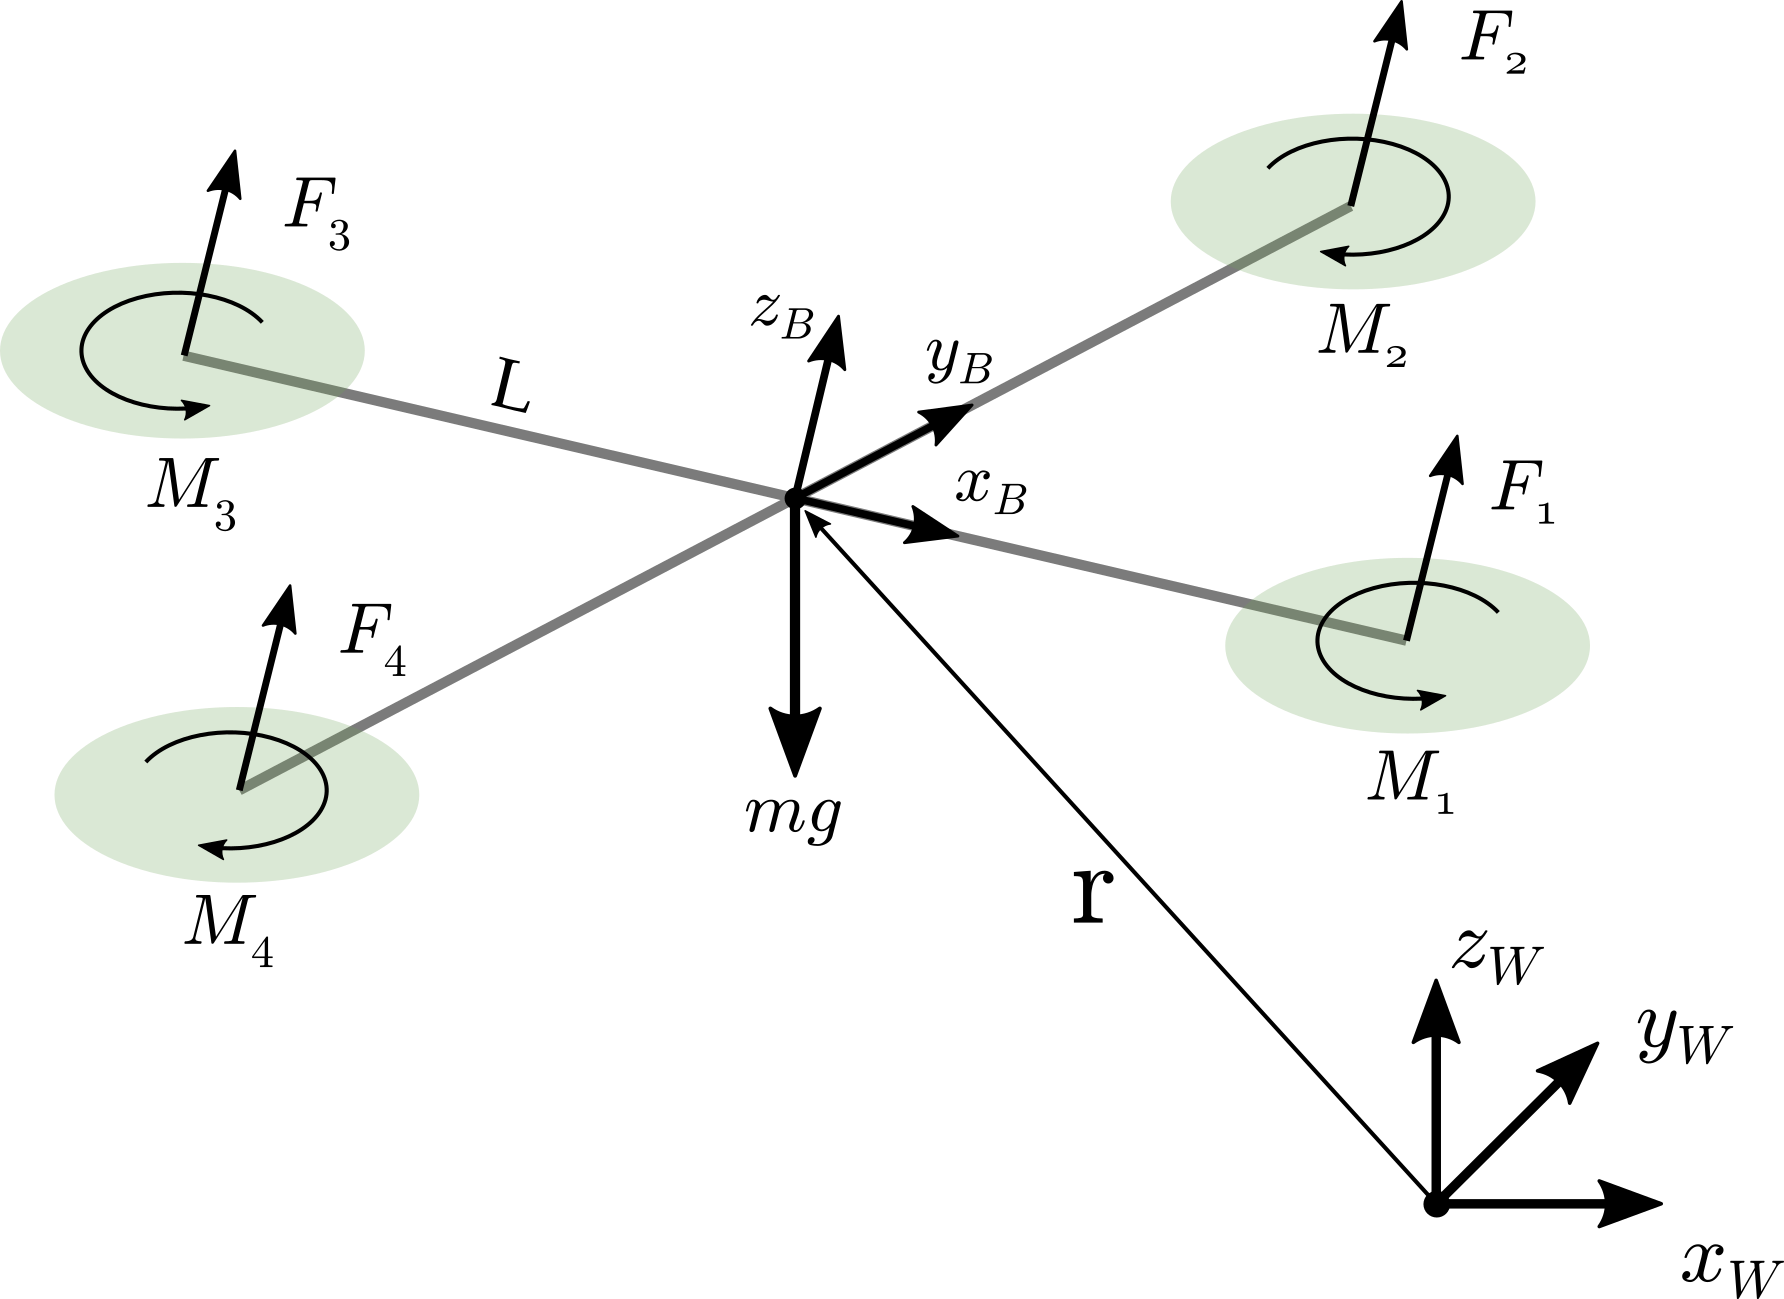
\includegraphics[width=0.65\textwidth]{imagenes/uav_coordinate_system}
	\caption{Esquema de fuerzas y momentos que actúan sobre un cuadricóptero y sus sistemas de referencia asociados. }
	\label{modelado:uav_coordinate}
\end{figure}

Como puede observar en la figura \ref{modelado:uav_coordinate}, se ha  empleado el subíndice $W$ para hacer referencia al sistema de referencia del mundo, así como el subíndice $B$ para referirse al sistema asociado al cuerpo del cuadricóptero. El \textit{frame} $B$ posee su origen $O_B$ en el centro de masas de la aeronave, con el eje $x_B$ coincidente con la dirección de avance preferente de la aeronave.

Para modelar las rotaciones del \textit{frame} $B$ con respecto a $W$ se emplearán los ángulos de Euler Z-X-Y, es decir, la matriz de rotación $R$ para transformar coordenadas desde $B$ a $W$ consiste en la composición de las siguientes rotaciones:
\begin{equation}
	R = R_{\mathbf{z},\psi}R_{\mathbf{x},\phi}R_{\mathbf{y},\theta}
	\label{modelado:euler_z_x_y}
\end{equation}
siendo $R_{\mathbf{i},\alpha}$ una rotación de un ángulo $\alpha$ respecto al eje $i$. Al desarrollar la expresión \ref{modelado:euler_z_x_y} se obtiene la matriz $R$ resultante
\begin{equation}
	\label{modelado:R}
	R = \begin{bmatrix}
		c_{\psi} c_{\theta} - s_{\phi} s_{\psi} s_{\theta} &  -c_{\phi} s_{\psi}& c_{\psi} s_{\theta} +  c_{\theta} s_{\phi} s_{\psi}\\
		c_{\theta} s_{\psi} +  c_{\psi} s_{\phi} s_{\theta} & c_{\phi} c_{\psi} & s_{\psi} s_{\theta} -  c_{\theta} s_{\phi} c_{\psi} \\
		-c_{\phi}s_{\theta}& s_{\phi} & c_{\phi}c_{\theta} 
	\end{bmatrix}
\end{equation}

donde $c_{\theta}$ y $s_{\theta}$ denotan $cos(\theta)$ y $sen(\theta)$ respectivamente.

En el sistema de referencia $B$ las componentes del vector velocidad angular $\Omega$ están definidas por $p$, $q$ y $r$ de la forma: 

\begin{equation}
	\Omega = p \mathbf{x_B} + q \mathbf{y_B} + r \mathbf{z_B}
\end{equation}

Estas componentes están relacionadas con las derivadas de los ángulos de Euler de acuerdo a

\begin{equation}
	\begin{bmatrix}
		p\\
		q\\
		r
	\end{bmatrix}  = \begin{bmatrix}
	c_{\theta}&0& -c_{\phi} s_{\theta}\\
	0 & 1 & s_{\phi}\\
	s_{\theta}&0 & c_{\phi} c_{\theta}
\end{bmatrix}\begin{bmatrix}
\dot{\phi}\\
\dot{\theta}\\
\dot{\psi}
\end{bmatrix} 
\end{equation}

\section{Análisis dinámico}
\subsection{Ecuaciones de movimiento traslacional}
Como se puede observar en la figura \ref{modelado:uav_coordinate}, las fuerzas que actúan sobre el cuadricóptero son: la gravedad, en la dirección $-\mathbf{z_W}$ y la fuerza de cada uno de los motores, en la dirección $\mathbf{z_B}$. Para hallar las ecuaciones que rigen la dinámica del centro de masas del sistema $C$ se aplican las ecuaciones de Newton sobre él. Siendo $\mathbf{r}$ el vector de posición del centro de masas $C$ con respecto al origen de $W$ obtenemos:

\begin{equation}
	\label{analisis:eq1}
	m \mathbf{\ddot{r}} = \begin{bmatrix}
		0\\
		0\\
		-mg
	\end{bmatrix} + R \begin{bmatrix}
	0\\
	0\\
	F_1+F_2 + F_3 + F_4
\end{bmatrix}
\end{equation}

Si denominamos $F  = \displaystyle\sum_{i=1}^{4}F_i$ , al expandir la ecuación anterior con la definición de $R$ en \ref{modelado:R} obtenemos las ecuaciones que describen el movimiento traslacional del centro de masas del cuadricóptero:

\begin{equation}
	\label{analisis:eq2}
	m \mathbf{\ddot{r}} = \begin{bmatrix}
		0\\
		0\\
		-mg
	\end{bmatrix} +\begin{bmatrix}
		s_{\theta}c_{\psi} + s_{\phi}c_{\theta}s_{\psi} \\
		s_{\theta}s_{\psi} - s_{\phi}c_{\theta}c_{\psi} \\
		c_{\phi}c_{\theta}
	\end{bmatrix} F
\end{equation}

\subsection{Ecuaciones de movimiento rotacional}

Como se puede observar en la expresión anterior, el movimiento del cuadricóptero depende de la rotación $R$, por lo que es necesario modelar el movimiento rotacional del mismo. Se define el momento angular $H$ como:
\begin{equation}
	H = \mathbf{I}\Omega
\end{equation}
donde $\mathbf{I} \in \mathbb{R}^{3\times 3}$ representa el tensor de inercia del cuadricóptero en el sistema $B$, y $\Omega  = [p, q, r]$ representa el vector de velocidad angular de $B$ respecto $W$. 

Si denotamos $M_c = [\tau_x, \tau_y, \tau_z]^t$ como el momento total del cuadricóptero en el sistema $B$

\begin{align}
	M_c &= \frac{d}{dt}H\nonumber\\
		&= \mathbf{I}\dot{\Omega}+\Omega\times\mathbf{I}\Omega
	\label{model:rot1}
\end{align}

Se considera que el cuadricóptero presenta una distribución de masa simétrica, por lo que el tensor de inercia $\mathbf{I}$ es un tensor diagonal de la forma:

\begin{equation}
	\mathbf{I} = \begin{bmatrix}
		I_{xx}&0&0\\
		0&I_{yy}&0\\
		0&0&I_{zz}\\
	\end{bmatrix}
\end{equation}
siendo $I_{xx}$, $I_{yy}$, $I_{zz}$ los momentos principales del cuadrícoptero con respecto a los ejes $x_B$, $y_B$, $z_B$ respectivamente.

Desarrollando la expresión \ref{model:rot1} y reorganizando sus términos:
\begin{align}
\mathbf{I}\begin{bmatrix}
	\dot{p}\\
	\dot{q}\\
	\dot{r}
\end{bmatrix}=
\begin{bmatrix}
	\tau_x\\
	\tau_y\\
	\tau_z
\end{bmatrix} -\begin{bmatrix}
	p\\
	q\\
	r
\end{bmatrix} \times\mathbf{I}\begin{bmatrix}
	p\\
	q\\
	r
\end{bmatrix}\label{model:rot2}
\end{align}

A partir del diagrama de la figura \ref{modelado:uav_coordinate} se puede calcular los valores de $\tau_x$, $\tau_y$ y $\tau_z$ a partir de las fuerzas y momentos ejercidos por los motores.

\begin{align}
	\tau_x &=  L (F_2-F_4)\nonumber\\
	\tau_y &=  L (F_3-F_1)\nonumber\\
	\tau_z &=  M_1 - M_2 + M_3 - M_4\label{model:rot3}
\end{align}

Finalmente se unen las expresiones \ref{model:rot2} y \ref{model:rot3} para obtener la ecuación de movimiento rotacional del cuadricóptero.






\begin{align}
	\mathbf{I}\begin{bmatrix}
		\dot{p}\\
		\dot{q}\\
		\dot{r}
	\end{bmatrix}=
	\begin{bmatrix}
		L (F_2-F_4)\\
		L (F_3-F_1)\\
		M_1 - M_2 + M_3 - M_4
	\end{bmatrix} -\begin{bmatrix}
		p\\
		q\\
		r
	\end{bmatrix} \times\mathbf{I}\begin{bmatrix}
		p\\
		q\\
		r
	\end{bmatrix}
\end{align}





\chapter{Control}


El problema del control se puede expresar formalmente: 
Dado el estado del sistema $x(t)$ \tb{continuar . ... }
como encontrar la función $u(t)$ tal que, el estado $x(t)$ sigue la trayectoria desesada $x^{des}(t)$ a lo largo del tiempo.\\
Si se define el error $e(t)$ del control como:
\begin{equation}
	e(t) = x^{des}(t) - x(t)
\end{equation}
el objetivo del controlador sería conseguir que el error $e(t)$ converja de forma exponencial a 0.


El estado $x(t)$ de un cuadricóptero consta de 12 variables, las 6 correspondientes a su pose y sus derivadas correspondientes.
\begin{equation}
	x(t) = \left[
	x  \;\;
	y  \;\;
	z  \;\;
	\phi  \;\;
	\theta  \;\;
	\psi  \;\;
	\dot{x}  \;\;
	\dot{y}  \;\;
	\dot{z}  \;\;
	\dot{\phi}  \;\;
	\dot{\theta}  \;\;
	\dot{\psi}\;\right]^t
\end{equation}
Si llamamos $q$ al vector de configuración formado por las 6 primeras variables:
\begin{align}
	q(t) &= \left[
	x  \;\;
	y  \;\;
	z  \;\;
	\phi  \;\;
	\theta  \;\;
	\psi  \;\right]^t\\
	x(t) &= \left[q \;\; \dot{q}\right]^t
\end{align}

\section{Controlador para ángulos pequeños}
Cuando las trayectorias que el cuadricóptero son poco agresivas se puede linealizar el modelo del cuadricóptero entorno a su punto de equilibrio. En la situación de equilibrio el cuadricóptero se encuentra en hover \textit{hover}, es decir manteniendo la posición en el aire. En \textit{hover} el estado $x_0$ de la aeronave es de la forma 
\begin{align}
	x_0 &= [q_0 \;\; 0]^t\nonumber\\
	q_0 &= [x  \;\;y  \;\;z  \;\;0  \;\;0  \;\;0  \;]^t
\end{align}


\section{Controlador para ángulos grandes}






	\chapter{Generación de trayectorias}\label{cap:gen_tray}

En el apartado anterior se ha diseñado un controlador cuyo objetivo es seguir una trayectoria deseada minimizando el error de seguimiento. En este apartado se tratará sobre la forma en la que se generan estas trayectorias. Este desarrollo se realiza entorno a una trayectoria unidimensional en un único eje de desplazamiento , el eje $x$. Este desarrollo es ampliable al espacio tridimensional realizando una trayectoria por cada eje.


\section{Trayectorias óptimas}\label{trajectoriasoptimas:cap}
El objetivo general del control óptimo es encontrar la función $x^*(t)$ que minimiza la expresión
\begin{equation}
	x^*(t) =  \underset{x(t)}{argmin}\int_{0}^{T}\mathcal{L}\left(x^{(n)},x^{(n-1)},...,\dot{x},x,t\right)\, dt
\end{equation}
siendo $\mathcal{L}$ el índice que se debe optimizar.

Cuando el objetivo es generar trayectorias suaves la forma de la expresión a optimizar es :
\begin{equation}
	x^*(t) = \underset{x(t)}{argmin}\int_{0}^{T}\left(x^{(n)}\right)^2\, dt
\end{equation}
siendo $x^{(n)} = u $, la magnitud de control que se desea minimizar. El valor del parámetro $n\in\mathbb{N}$, expresa el grado de la derivada de la acción de control $u$, es decir, para generar trayectorias de mínima distancia, se empleará un valor de $n=1$, por lo que $u = \dot{x}$, mientras que para generar trayectorias de mínima sobreacceleración (\textit{jerk}) se empleará un valor de $n=3$, por lo que $u = \dddot{x}$.

De forma general la expresión a optimizar será:
	\begin{equation}
		x^*(t) = \underset{x(t)}{argmin}\int_{0}^{T}\mathcal{L}\left(x^{(n)}, x^{(n-1)},...,\dot{x},x,t\right)\, dt
	\end{equation}

De la  ecuación de Euler-Lagrange se obtiene que la la función ófptima $x^*(t)$ debe satisfacer:
\begin{equation}
	\frac{\partial\mathcal{L}}{\partial x} + \sum_{i=1}^{n}(-1)^i \frac{d^i}{dt^i}\left(\frac{\partial\mathcal{L}}{\partial x^i}\right)  = 0
\end{equation}
Si particularizamos la expresión anterior a expresiones donde $\mathcal{L} =\left(x^{(n)}\right)^2$, todos las derivadas parciales $\frac{\partial\mathcal{L}}{\partial x^i} = 0 \; ; \forall i \neq n$ por lo que:
\begin{align}
	\frac{d^n}{dt^n}\left(\frac{\partial\mathcal{L}}{\partial x^n}\right) = 0 \\
	\frac{d^n}{dt^n}\left(2 x^{(n)}\right) = 0\\
	x^{(2n)} = 0
\end{align}
Al integrar la expresión anterior se obtiene el polinomio de grado $2n-1$, con $2n$ coeficientes:
\begin{equation}
	x(t) = c_{2n-1}t^{2n-1} + c_{2n-2}t^{2n-2} + ... + c_2t^2 + c_1t + c_0
\end{equation}
Para resolver los coeficientes, son necesarias $2n$ condiciones de contorno que corresponden con los valores de la función $x(t)$ y de sus derivadas en los instantes $t=0$ y $t = T$. Si se considera que la trayectoria transcurre entre un estado inicial y un estado final, ambos estados de equilibrio , se puede considerar que las derivadas son nulas por lo que las condiciones de contorno serían:
\begin{align}
 	&x(0) = a; \quad \;\dot{x}(0) = 0;  \quad...\quad x^{(2n-1)}(0) = 0\\
	&x(T) = b;\quad \dot{x}(T) = 0;  \quad...\quad x^{(2n-1)}(T) = 0
\end{align}
Con estas condiciones de contorno se calcula la trayectoria óptima para pasar de una posición inicial $a$ a una posición final $b$ en un tiempo $T$ minimizando la acción de control $u = x^{(n)}$. 



\section{Trayectorias continuas a trozos}
Para generar trayectorias que el cuadricóptero deba seguir para completar el circuito es conveniente contar con puntos de paso (\textit{waypoints}) por los que se quiere que pase el aeronave, por ejemplo, el centro de las puertas (Figura \ref{TrajCont}).


\begin{figure}[htb!]
	\centering
	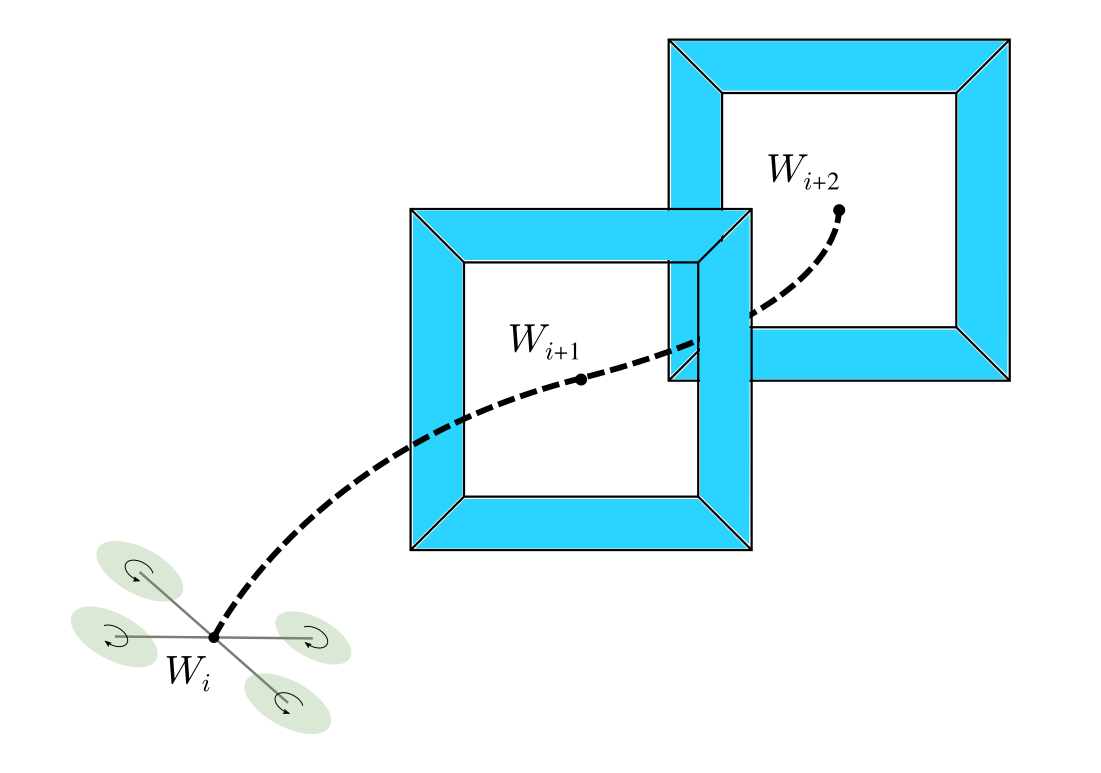
\includegraphics[width=0.7\textwidth]{imagenes/TrajCont}
	\caption{Esquema del objetivo de la generación de trayectorias empleando como waypoints los centros de las puertas y la posición del aeronave.}
	\label{TrajCont}
\end{figure}

Como se puede observar en el apartado anterior, las trayectorias que se generan entre dos puntos de paso $a$ y $b$, son trayectorias polinómicas cuyo grado depende del orden de la derivada de la acción de control. Debido a esto, se ha decidido usar trayectorias de tipo \textit{spline}, es decir, curvas diferenciables definidas en segmentos polinómicos, donde cada segmento sería una trayectoria entre dos \textit{waypoints}. Cada trayectoria completa, $r_d(t)$ está compuesta por $m$ segmentos de grado $q$, presentando la estructura

\begin{equation}
	r_d(t) = \left\{ 
	\begin{array}{ll}
		\sum_{i=0}^{q}a_{i1}t^{i} &,t_0\leq x \leq t_1 \\
		\sum_{i=0}^{q}a_{i2}t^{i} &,t_1\leq x \leq t_2 \\
		\qquad\vdots &\qquad\vdots \\
		\sum_{i=0}^{q}a_{im}t^{i} &,t_{m-1}\leq x \leq t_m \\
	\end{array}
	\right.
\end{equation}

siendo $a_{ij}\in \mathbb{R}$ los coeficientes de los polinomios. El grado $q$ de estos polinomios dependerá del índice a minimizar durante el transcurso de la trayectoria, como se ha explicado en el apartado \ref{trajectoriasoptimas:cap}. Cada tramo tiene un tiempo inicial y un tiempo final, estos tiempos dependen de las limitaciones físicas del aeronave, es decir, de su velocidad y aceleración máximas, en el apartado \ref{sec:estimacion_tiempos} se profundiza en la forma de generar estos tramos temporales.

De cara a resolver el valor de los distintos coeficientes de cada segmento polinomial se emplearán unas condiciones de contorno que garanticen la derivabilidad de la trayectoria completa en las $q$ primeras derivadas. 

Si se considera una trayectoria completa a través de $n$ \textit{waypoints} $P$ distribuidos a lo largo del tiempo, siendo $t_0$ el tiempo inicial del primer segmento y $t_n$ el tiempo final de la trayectoria, la trayectoria contará con $n-1$ segmentos polinómicos $S$ de grado $q$. Considerando que en el punto inicial y el punto final de la trayectoria el cuadricóptero se encuentra en un estado de equilibrio, las condiciones de contorno empleadas para calcular los coeficientes de la \textit{spline} son:
\begin{equation}
\begin{array}{ll}
	S_i (t = t_{i-1}) = W_{i-1} \quad &\forall i \in 1,...,n\\
	S_i (t = t_{i}) = W_i \quad &\forall i \in 1,...,n\\
	S_1^{(k)}(t = t_0) = 0 \quad &\forall k \in 1,...,q\\
	S_n^{(k)}(t = t_n) = 0 \quad &\forall k \in 1,...,q\\
	S_{i-1}^{(k)}(t = t_{i-1}) = S_{i}^{(k)}(t = t_{i})  \quad &\forall k \in 1,...,q \;; \forall n \in 2,...,n
\end{array}
\end{equation}
 siendo $W_i$ la posición del i-ésimo \textit{waypoint} , $S_i$ el i-ésimo segmento polinómico y  $t_i$ el tiempo de finalización del segmento $S_i$.
 
 Las dos primeras condiciones de contorno hacen referencia a las posiciones espaciales de los waypoints, es decir, que cada segmento empiece en un waypoint  y termine en el siguiente. Las dos condiciones siguientes hacen referencia al valor de las derivadas en los estados iniciales y final, se ha considerado que los estado inicial y final, son estados de equilibrio por lo que el valor de sus derivadas es nulo. Finalmente la ultima condición hace referencia a la continuidad de las derivadas entre segmentos, es decir, que el valor de las derivadas del final de un segmento, sean iguales al las derivadas iniciales del segmento siguiente, de esta forma se consigue que la trayectoria completa generada cumpla la condición de derivabilidad a lo largo de todas sus $q$ derivadas.

\section{Estimación de tiempos}\label{sec:estimacion_tiempos}

El objetivo final es generar trayectorias a través del circuito de forma que el aeronave sea capaz de recorrerlas teniendo en cuenta restricciones de posición, velocidad y aceleración. En los dos apartados anteriores se explica como generar trayectorias óptimas teniendo en cuentas restricciones de posición, fijando los \textit{waypoints} por los que se desea que pase el cuadricóptero. Sin embargo, para poder generar trayectorias es también necesario elegir los segmentos temporales $T_i$ entre los distintos puntos de paso, es decir, los tiempos que debe tardar el aeronave en pasar entre los distintos waypoints. Estos segmentos de tiempo deben tener en cuenta las limitaciones de velocidad y acceleración máximas del aeronave, para poder generar trayectorias realizables. A continuación se tratará un posible método para establecer la duración de estos intervalos temporales.

\subsubsection{Aproximación al tiempo medio}

La forma más sencilla de establecer intervalos temporales es basarse en la distancia existente entre un par de waypoints y la velocidad media a la que se desea que vuele el aeronave para estimar el tiempo necesario. Siendo $d_i = || W_{i-1} , W_{i} ||_2 $ la distancia entre dos \textit{waypoints} consecutivos y $v_m$ la velocidad media de vuelo, se puede establecer la duración de un segmento $S_i$ como
\begin{align}
	T_i = \frac{d_i}{v_m}
\end{align}
Para obtener los valores de tiempo absoluto $t_i$ requeridos en el apartado anterior simplemente se deben sumar las duraciones de los segmentos anteriores.
\begin{align}
t_i = \sum_{j=1}^{i} T_j
\end{align}


Para tener aumentar el control sobre la agresividad de la trayectoria se puede añadir un coeficiente $\alpha_i$ que permita modificar ligeramente el valor $T_i$ siendo 
\begin{align}
	T_i = \alpha_i\frac{d_i}{v_m}
\end{align}

Valores de $\alpha_i$ pequeños generan trayectorias más agresivas, así como valores más grandes producen trayectorias más seguras. Iterando el valor de este parámetro $\alpha_i$ se controla que las limitaciones en velocidad y aceleración máxima se cumplan para cada segmento $S_i$.

Esta es una forma simple y rápida de establecer los distintos segmentos temporales, sin embargo, es una aproximación que afecta a la generación de la trayectoria óptima, haciendo que el tiempo total que se tarda en recorrer el circuito sea mayor que el que se podría obtener usando otros métodos de optimización como los propuestos por Mellinger et al. \cite{MinimunSnap2011} o por Foehn. et al. \cite{foehn2020cpc}  para la obtención de estos segmentos temporales. A pesar de esto, debido a que las posiciones de los \textit{waypoints} cambian rápidamente a lo largo del circuito y se deben recalcular las trayectorias continuamente, el bajo coste computacional que presenta este método hace que merezca la pena su utilización.


	\chapter{Metodología}
	
\tb{En los capítulos anteriores se ha presentado los distintos algoritmos de control y generación de trayectorias que se emplearñan para conseguir recorrer un circuito con un \tb{dron} de carreras autónomo }. En este apartado se presenta la metodología empleada para superar las pruebas clasificatorias del Alphapilot 2019 

\section{Sistemas de referencia}


\section{Generación de \textit{waypoints}}
Para recorrer el circuito de forma satisfactoria es necesario que la aeronave atraviese las distintas puertas o \textit{gates} que componen el circuito en un orden concreto. Para conseguir esto es necesario conocer las posiciones de las puertas en el mundo y generar los puntos de paso necesarios para que la aeronave pase a través de ellas sin colisionar.

En la competición se proporciona el orden en el que se deben atravesar las puertas y una posición aproximada de las posiciones de cada una de ellas en el mundo. 

\begin{figure}[htb!]
	\centering
	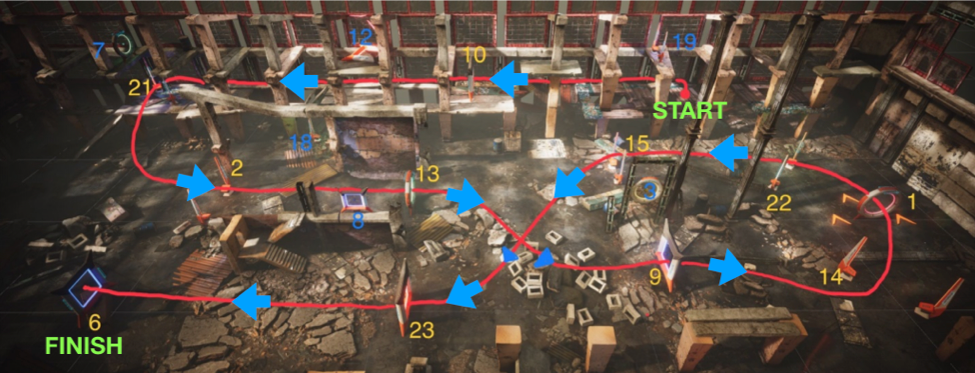
\includegraphics[width=\textwidth]{imagenes/diagramacircuito}
	\caption{Vista aérea del circuito en el simulador FightGoggles, las puertas que se deben traspasar se simbolizan con su número en color amarillo.}
	\label{waypoints:circuito}
\end{figure}

Como se puede observar en la figura \ref{waypoints:circuito} la aeronave debe recorrer 11 puertas, cada una con un número de identificación, en el orden indicado. 








\section{Trayectorias a largo y corto plazo}


	\chapter{Arquitectura del sistema}

Para conseguir que los distintos módulos que integran el sistema trabajen de forma conjunta es necesario establecer una arquitectura que permita la comunicación eficiente entre ellos así. Para coordinar el trabajo de los distintos módulos que componen el sistema se ha empleado ROS (\textit{Robot Operating System}) \cite{ros} un \textit{framework} orientado a el desarrollo de software para robots ampliamente extendido en la comunidad robótica. En el paradigma de ROS el código se estructura en nodos independientes que se comunican entre ellos a través de tópicos (mensajes que un nodo difunde de forma general a los demás nodos y cualquiera lo puede leer) y servicios (peticiones de un nodo particular a otro).

Esto permite desarrollar cada componente del sistema de forma independiente y comunicarlos entre ellos mediante una interfaz común. Esto permite encapsular el código, lo que aumenta la reusabilidad y la robustez de cada módulo, independiente del resto de módulos que les rodeen.

A continuación se explicará más detalladamente los distintos nodos que componen la arquitectura:
\begin{itemize}
	
	\item \textbf{Simulador:} En la arquitectura propuesta el entorno de simulación empleado, Flightgoogles, se comporta como un nodo adicional. Este nodo constituye el interfaz de comunicación entre la aeronave simulada y el entorno simulado,
	el cual publica datos sobre el estado de la aeronave como su posición y orientación, las imágenes de las cámaras simuladas y la posición de las esquinas de las puertas en las imágenes obtenidas. Asimismo, recibe los comandos de control enviados a la aeronave.
	 
	\item \textbf{Estimación de estado.} Este modulo se encarga de completar la estimación de estado de la aeronave, empleando la información temporal sobre los cambios de pose de la aeronave. Además proporciona esta información a través de mensajes estándar al resto de los módulos de la arquitectura.
	
	\item \textbf{Percepción.} El simulador provee las imágenes, tomadas por las cámaras, del entorno simulado. En estas imágenes aparecen las puertas del circuitos con un indicador del número de puerta, así como las posiciones de las esquinas de las puertas en las imágenes tomadas. Conociendo los parámetros de la cámara y las dimensiones de las puertas se puede extrapolar la posición de las puertas respecto a la cámara. El modulo de percepción se encarga de enviar las posiciones aproximadas de las distintas puertas del circuito e ir actualizando estas estimaciones a medida que la aeronave avanza a través del circuito.
	
	\item \textbf{Generador de trayectorias.} Una vez conocida la posición de la aeronave en el circuito y las posiciones aproximadas de las puertas con respecto a la aeronave se genera la trayectoria que debe seguir la aeronave para pasar a través de las puertas de la forma más rápida posible sin colisionar con el entorno. Para poder actualizar la trayectoria de forma rápida con un coste bajo computacional se divide este trabajo en dos módulos:
	
	\begin{itemize}
		\item \textbf{Trayectoria a largo plazo}: Obtiene las posiciones de las puertas provistas por el módulo de percepción y genera el recorrido tridimensional completo que debería realizar el cuadricóptero. 
		
		\item \textbf{Trayectoria a corto plazo}: Recibe la trayectoria a largo plazo y la evalúa en un corto horizonte temporal respecto a la posición actual de la aeronave. Dentro de este horizonte se genera la trayectoria de control óptima a seguir. Este módulo también se encarga de evaluar la trayectoria actual a lo largo del tiempo y enviar las consignas de posición, velocidad y aceleración al controlador.
	\end{itemize}
	
	\item \textbf{Controlador:} El módulo del controlador recibe el estado actual de la aeronave provisto por el modulo de estimación y la referencias provistas por el módulo trayectoria a corto plazo. Con esto genera las acciones de control que se envían al módulo del simulador.
	
\end{itemize}

\tb{\Large Añadir Diagrama de la arquitectura con los topics involucrados.}

\section{Detalles de implementación}

Todos los algoritmos desarrollados se han implementado en C++17 haciendo uso tanto de las librerías estándar como de las librerías estándar de ROS . Además se ha hecho uso de algunas librerías específicas como OpenCV 4.0 para el tratamiento de las imágenes, así como Eigen3 para computar las operaciones matriciales requeridas por los algoritmos implementados. A continuación, se explicarán algunos detalles de implementación relevantes de los distintos módulos.

\subsection{Módulo de control}

Para facilitar el ajuste de las ganancias de los distintos controladores se ha empleado la librería de ROS \textit{dynamic reconfigure}. Esta librería permite variar el valor de distintos parámetros en tiempo de ejecución, lo que facilita enormemente el ajuste fino de los parámetros de los controladores. 
\tb{\Large Imagen Dynamic Reconfigure}
\newpage
\subsection{Módulo de generación de trayectorias}

Dado que las dos trayectorias generadas, la de corto y la de largo plazo, se generan empleando \textit{splines} se ha unificado el algoritmo de generación en una clase común a ambos módulos. Aunque al comienzo del proyecto se empleo una implementación propia de estos algoritmos, finalmente se ha optado por emplear la implementación realizada por la ETHZ (disponibles para la comunidad robótica en \url{https://github.com/ethz-asl/mav_trajectory_generation}) debido a que alcanzaban una mayor eficacia en la generación de las mismas.

Adicionalmente, debido a que el módulo generador de trayectorias a corto plazo es el encargado también de generar las referencias del controlador ha sido necesario paralelizar la generación de las trayectorias y la evaluación de las mismas a lo largo del tiempo. Es por eso que se ha separado la computación en dos hilos diferentes: un hilo principal que se encarga de muestrear la trayectoria generada a una alta frecuencia (100 Hz) y de enviar las referencias al controlador y un hilo secundario que se encarga de generar la siguiente trayectoria a corto plazo a seguir.

\tb{\Large Pequeña imagen de los hilos}





	\chapter{Experimentos}

\begin{figure}[htb!]
	\centering
	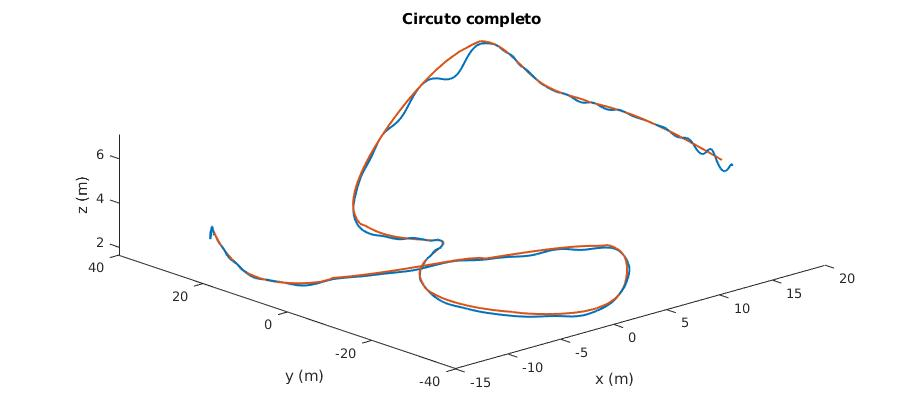
\includegraphics[width=\textwidth]{imagenes/circuitFigure}
	\caption{}
	\label{exp1:1}
\end{figure}

\begin{figure}[htb!]
	\centering
	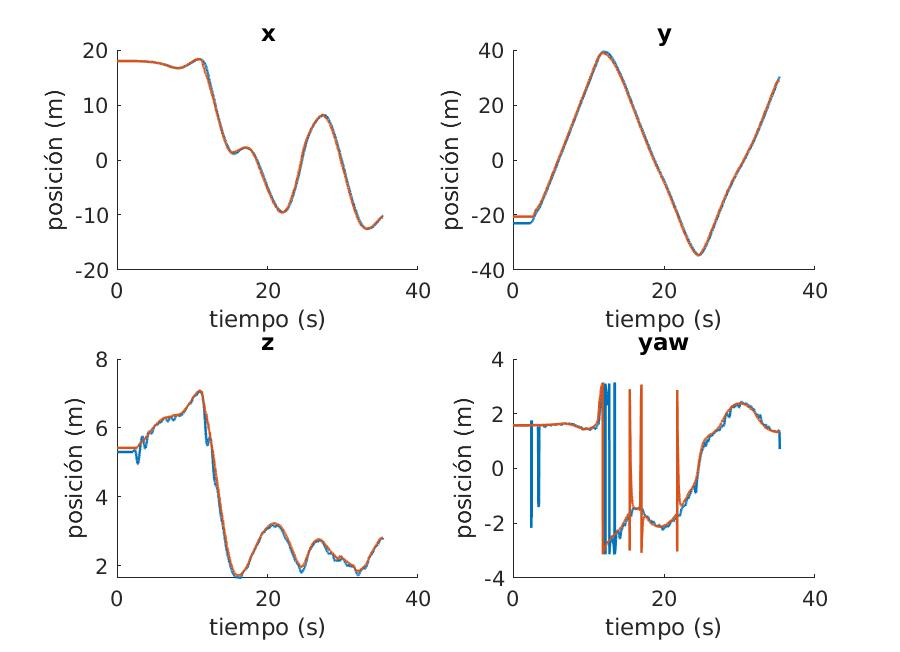
\includegraphics[width=\textwidth]{imagenes/positionFigure}
	\caption{}
	\label{exp1:2}
\end{figure}

\begin{figure}[htb!]
	\centering
	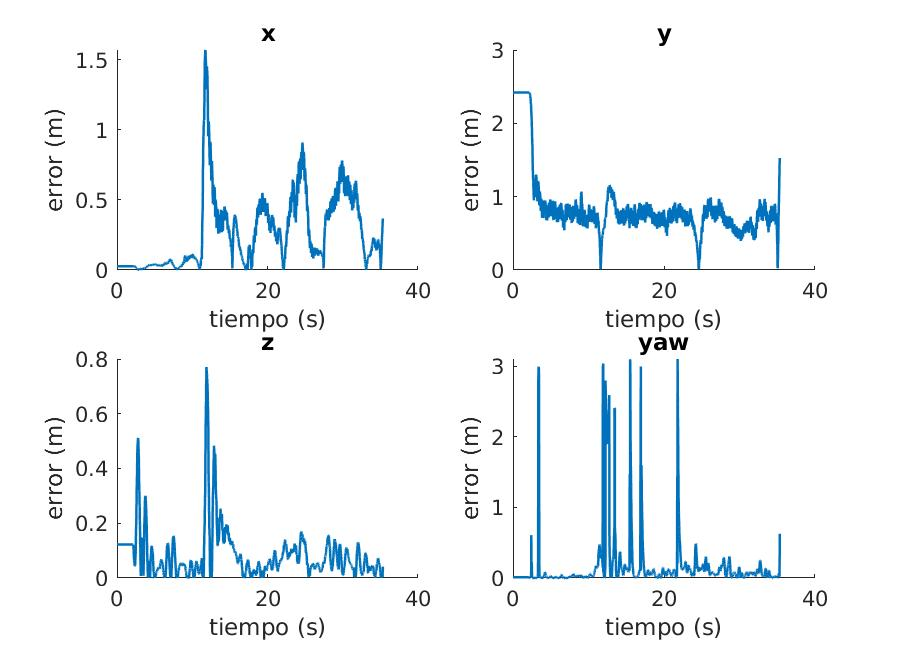
\includegraphics[width=\textwidth]{imagenes/errorFigure}
	\caption{}
	\label{exp1:3}
\end{figure}

\begin{table}[htb!]
	\centering

\begin{tabular}{l|c|c|c|}
	$\empty$&Eje x&Eje y&Eje z\\
\midrule
	Error máximo (m)&1.5685&1.1577&0.7707\\
	Error medio (m) &0.3143&0.7306&0.0796\\
	
\end{tabular}
\caption{Errores de seguimiento durante el recorrido del circuito.}
\end{table}

\section{Experimentos en simulación}
\section{Experimentos en real}
	%\chapter{Discusión}


	\chapter{Conclusiones y trabajo futuro}

\section{Conclusiones}

Durante el transcurso de este trabajo se ha desarrollado la arquitectura modular para un cuadricóptero de carreras autónomo. Esta modularidad de la arquitectura ha facilitado el desarrollo de los algoritmos de forma aislada así como el desarrollo de los experimentos de control, en los que se ha podido intercambiar los módulos de generación de trayectorias por módulos más sencillos de forma ágil. Esta modularidad también permitiría sustituir el módulo del simulador por un módulo de interfaz con una plataforma real, lo que facilitaría la realización de experimentos en real.

En cuanto al control del cuadricóptero se han conseguido implementar dos controladores del estado del arte de forma satisfactoria adaptándolos a las señales de control requeridas por el cuadricóptero. El empleo de herramientas como el \textit{dynamic reconfigure} de ROS han permitido realizar el ajuste de las ganancias de los controladores \textit{online}, lo que ha reducido considerablemente los tiempos necesarios para realizar estos ajustes.

Por otro lado, la decisión de separar la generación de trayectorias en dos partes, una a largo plazo y otra a largo plazo, ha permitido generar trayectorias de control óptimas en \textit{snap} con una alta reactividad frente a los cambios en las estimaciones de las puertas, manteniendo un bajo coste computacional en la generación de ambas trayectorias.

Finalmente, se han validado los desarrollos e implementaciones realizados en un entorno de simulación fotorrealista, consiguiendo completar el circuito de carreras completo de forma satisfactoria con una velocidad máxima de vuelo de 10,5 m/s en un tiempo inferior a los 23 segundos, lo que se situaría dentro de los mejores obtenidos el año pasado durante las clasificatorias virtuales del AlphaPilot2019.



\section{Trabajo futuro}

El trabajo realizado deja una arquitectura modular que permite su ampliación con nuevos módulos para adecuarla a la realización de distintas tareas de forma sencilla. Para una utilización del sistema en un caso real sería necesario implementar los módulos de estimación y percepción del entorno de una forma integral, empleando únicamente las medidas obtenidas por los sensores de la aeronave. 

Para mejorar el comportamiento del controlador sería conveniente emplear un controlador predictivo basado en el modelo (MPC), que permitiría reducir el error de seguimiento suavizando las acciones bruscas realizadas por el controlador cuando sufre cambios en la trayectoria de referencia. Junto con este controlador, se podrían emplear algoritmos de auto-identificación que permitan estimar \textit{online} el valor de los parámetros dinámicos de la aeronave, así como identificar posibles perturbaciones presentes en el entorno como podría ser el viento.

Finalmente, se podrían implementar métodos de optimización para calcular trayectorias que tengan en cuenta restricciones espaciales, lo que permitiría su empleo en entornos complicados con obstáculos alrededor. 












	\appendix
 
\chapter{Presupuesto y Planificación}

\section{Presupuesto}

El presupuesto del trabajo se puede separar en dos partes: recursos humanos y amortización de los equipos utilizados.

En cuanto a los recursos humanos empleados, se ha tenido una dedicación por parte del alumno de unas 400 horas, lo que se corresponde dentro del número de horas de dedicación esperadas en la realización de un Trabajo fin de Máster (12 ECTS). Un salario mensual de ayudante investigador a jornada completa en la universidad, es de unos 1250 euros, lo que se traduce en un coste de unos 8,33 euros la hora. El salario del tutor se ha extraído del portal de transparencia de la UPM. La dedicación del tutor ha sido de unas 30 horas de implicación en el trabajo.

\begin{figure}[htb!]
		\centering
		\begin{tabular}{|l|r|r|r|}
		\hline
		%\textbf{Recursos humanos} &Coste unitario [EUR] &Unidades&Total [EUR]\\
		
		\textbf{Recursos humanos} & Horas &Coste Horario [EUR]&Total [EUR]\\
		\hline
		
		Alumno & 400 & 8.33 &  3332 \\
		Tutor & 30& 33.72 & 1011.6 \\
		\hline
		\textbf{Total} & &  & \textbf{4343.6}\\
		\hline
		\end{tabular}\\
	
\end{figure}


En cuanto a la amortización del equipo, se ha empleado un ordenador para el desarrollo del software y para la realización de los experimentos. Se ha considerado una amortización lineal del 10 \% de la vida útil (4 años).

\begin{figure}[htb!]
	\centering
	\begin{tabular}{|l|r|r|r|}
		\hline
		\textbf{Equipo} & Precio &Coste Amortización(10\%)\\
		\hline
		Pc sobremesa & 1980 & 198\\
		\hline
		\textbf{Total} & & \textbf{198}\\
		\hline
\end{tabular}\\
\end{figure}

Con lo que el coste total del proyecto ha sido:

\begin{figure}[htb!]
	\centering
	\begin{tabular}{|l|r|r|r|}
		\hline
		\textbf{Concepto} &Total [EUR]\\
		\hline
		Recursos humanos & 4343.6\\
		Amortización del equipo & 198\\
		
		\hline
		\textbf{Total}   & \textbf{4541.6}\\
		\hline
	\end{tabular}\\
\end{figure}




\newpage
\section{Planificación}
La realización de este trabajo ha empleado un ritmo continuo de horas de trabajo desde su comienzo, a comienzos de abril. La dedicación media invertida en el desarrolo del trabajo ha sido de unas 35 horas semanales, durante un periodo de unos 3 meses, lo que da un total de unas 400 horas. El trabajo se ha realizado dentro del grupo de investigación CVAR (\textit{Computer Vision and Aerial Robotics}) del departamento de Electrónica Automática e Informática industrial de la Escuela Técnica Superior de Ingenieros Industriales (ETSII) perteneciente a la Universidad Politécnica de Madrid (UPM).

En cuanto a la distribución del trabajo en este tiempo, el trabajo comenzó a realizarse a finales de abril de 2020, durante el primer mes se realizó el curso sobre robótica aérea de UPenn, en la plataforma \textit{online} Coursera. La duración del curso se extendió hasta finales de abril. En mayo el trabajo se focalizó en el desarrollo de la arquitectura que se emplearía posteriormente, así como en el estudio del arte de los diferentes algoritmos de control y métodos de generación de trayectorias relevantes en el campo a estudiar. En junio y julio, se realizaron las implementaciones de los distintos algoritmos y se realizaron los primeros experimentos. Finalmente se ha redactado la memoria del proyecto en el mes de Septiembre. Se ha realizado un diagrama GANTT (\cref{gantt}) en el que se ha detallado más en profundidad la distribución temporal de las tareas. Asimismo, se ha esquematizado la organización del proyecto en un diagrama EDP 


\begin{figure}[htb!]
	\centering
	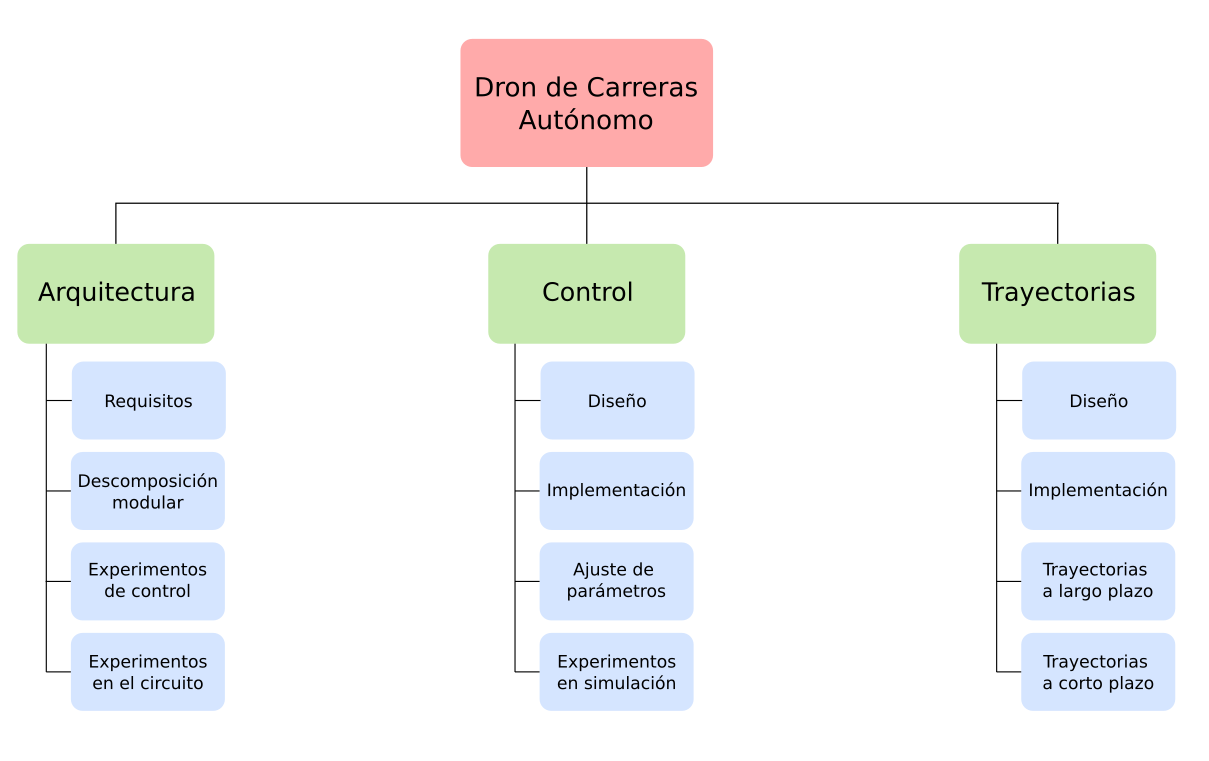
\includegraphics[width=0.85\textwidth]{imagenes/EDP}
	\caption{Diagrama EDP}
	\label{edp}
\end{figure}

\newpage

\textcolor{white}{aligment}
\begin{figure}[htb!]
	\centering
	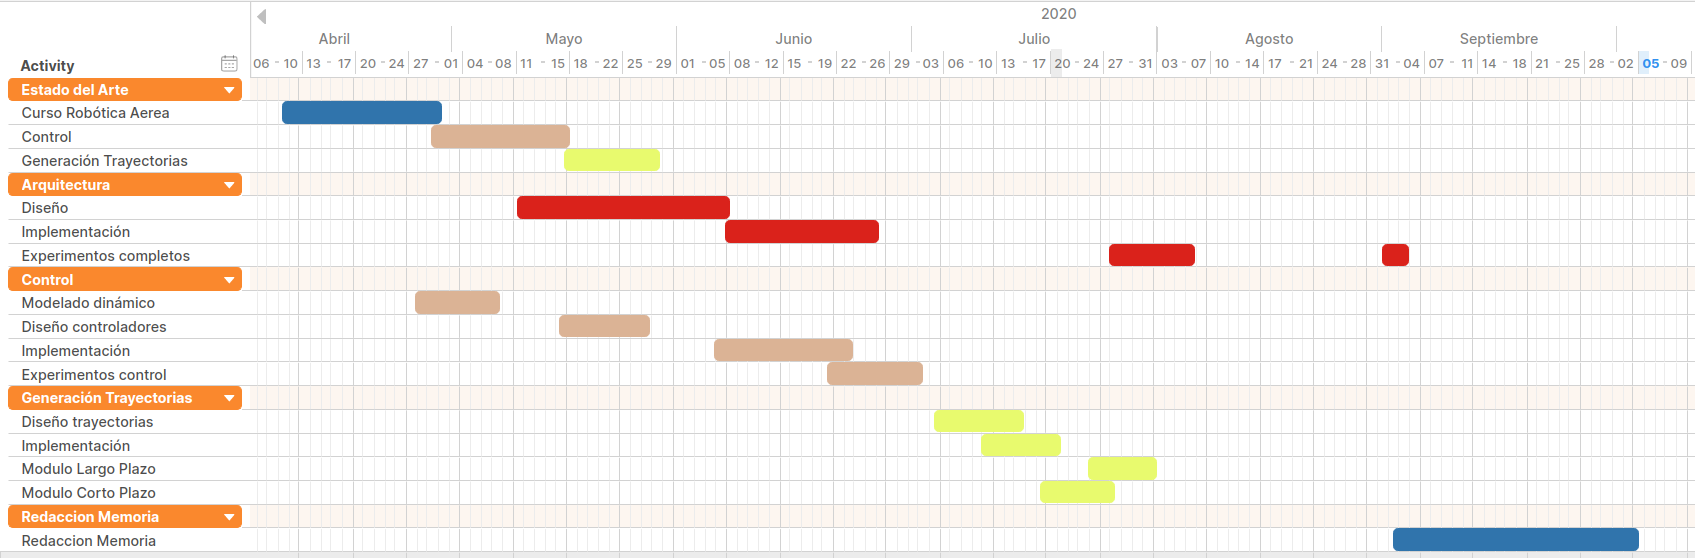
\includegraphics[angle=90,width =0.45\textwidth]{imagenes/gantt}
	\caption{Diagrama Gantt}
	\label{gantt}
\end{figure}


	
%	\pagenumbering{arabic}
%	
	\newpage
	\listoffigures
	\listoftables
		\nocite{*}
	\bibliographystyle{bibliografia/IEEEtran}
	\bibliography{bibliografia/IEEEabrv,bibliografia/workBibliography}
	
\end{document}
